\documentclass[11pt]{article}
\usepackage[margin=2.2cm]{geometry}
\usepackage{amsmath,amssymb,tikz,booktabs}
\usetikzlibrary{arrows.meta}
\title{Production regions as decay-like triangles: plan}
\date{}
\begin{document}
\maketitle

\paragraph{Goal.} Evaluate the 579 iterated-integral generators, and hence the 84 finite remainders, in the three
production regions $x>1$, $y>1$, $z>1$ (the other two variables negative). We use the same differential equation and the
same numerical method as in the decay region, and the same series pipeline. Crossings of the partons come later.

\paragraph{1. Bounding the regions.} In region $A>1$ the large variable is the energy. We write $A=1/v$ and the
other two as $-\hat b/v$, $-\hat c/v$, so that $\hat b+v+\hat c=1$ with $\hat b,\hat c,v>0$. The region becomes a
triangle, and $v$ is always the inverse energy. For example, for $z>1$: $x=-w/v$, $y=-u/v$, $z=1/v$, and
$(X,Y,Z)=(w,u,v)$ plays the role of $(x,y,z)$. These are the same variables as the continued-region charts of the
boundary-constant transport.

\paragraph{2. The alphabet closes.} Substituting the map into the twenty letters, every letter becomes a constant
times a power of $v$ times a letter of the same alphabet in $(X,Y)$. The odd letters need the continued root
$\sqrt{xyz}\to-\sqrt{XYZ}/Z^2$, and then
\[ d\log W_7\to d\log W_7'+d\log W_8',\qquad d\log W_8\to -d\log W_8' . \]
For $z>1$ the even letters map as follows:

\begin{center}
\begin{tabular}{@{}cccccccccccc@{}}\toprule
$W_1$&$W_2$&$W_3$&$W_4$&$W_5$&$W_6$&$W_{11}$&$W_{12}$&$W_{13}$&$W_{14}$&$W_{15}$&$W_{16}$\\
$W_1'/v$&$W_2'/v$&$1/v$&$W_5'/v$&$W_4'/v$&$W_6'/v$&$W_{12}'/v^2$&$W_{11}'/v^2$&$W_9'/v^2$&$W_{18}'/v^2$&$W_{17}'/v^2$&$W_{10}'/v^2$\\\bottomrule
\end{tabular}
\end{center}

So in the region $dF=\sum_j d\log W_j'\,M_j'F$, with $M_j'=\sum_k c_{kj}M_k$ and $c_{kj}$ integers. It is the same
system on a triangle, and the same integrator applies.

\paragraph{3. The continuation sits in the boundary values.} The corner $X,Y\to0$ of the region's triangle is the
attached decay corner, approached from the other side: $c_1$ for $z>1$, $c_2$ for $x>1$, $c_3$ for $y>1$. Going from
one side to the other is a half-turn around the corner. In the blow-up chart variables of that corner the Feynman
prescription gives
\[ \log t\to\log t-i\pi,\qquad \log B\to\log B+i\pi . \]
Chen's formula across the corner then reads
\[ \mathrm{II}[a_1\dots a_n](P)=\sum_k \mathrm{II}[a_1\dots a_k](P^*)\;\mathrm{II}'_{P^*\to P}[a_{k+1}\dots a_n] , \]
where:
\begin{itemize}
\item the values at the corner, $\mathrm{II}[\dots](P^*)$, are the logarithmic part of the decay expansion at the
  corner with the substitution above. They are polynomials in $i\pi$ (and MZVs at $c_2$, $c_3$), and in general
  nonzero;
\item the remaining factors are iterated integrals in the new variables, starting at the corner, so they vanish there
  (regularised).
\end{itemize}
At the level of the whole system: the start values at the new corner are these polynomials instead of zero, and the
connection is $M'$. Inside the triangle nothing is crossed, so no $i0$ is needed along the paths.

\begin{center}
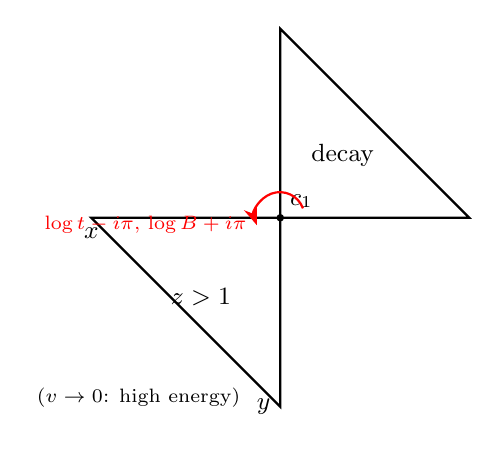
\begin{tikzpicture}[scale=2.4,>=Stealth]
  \draw[thick] (0,0)--(1,0)--(0,1)--cycle; \node at (0.33,0.33) {\small decay};
  \fill (0,0) circle (0.02) node[above right] {\small $c_1$};
  \draw[thick] (0,0)--(-1,0)--(0,-1)--cycle;
  \node at (-0.42,-0.42) {\small $z>1$}; \node at (-0.75,-0.95) {\scriptsize ($v\to0$: high energy)};
  \draw[->,red,thick] (0.12,0.05) arc (20:200:0.13) node[left] {\scriptsize $\log t-i\pi$, $\log B+i\pi$};
  \node[below] at (-1,0) {\small $x$}; \node[left] at (0,-1) {\small $y$};
\end{tikzpicture}
\end{center}

\paragraph{4. What we compute.} For each region:
\begin{itemize}
\item the integer letter map $c_{kj}$;
\item the connection $M'$, in the orthonormal gauge of the evaluator;
\item the values at the corner from the ITER series at the attached decay corner (exact);
\item the series start from the corner, carried to a hub $P_0'=(0.3,0.3)$ of the region's triangle, and stored;
\item evaluation of the generators and of the remainders. The rational functions are evaluated at the physical point,
  and $r=-\sqrt{|xyz|}$.
\end{itemize}

\paragraph{Checks.}
\begin{enumerate}
\item The generators at points of the region: the region evaluator against a direct integration from the decay hub
  $P_0$, crossing $x=0$ and $y=0$ from above. These are two independent continuations.
\item The leading-colour layer against the production-channel files of the 2024 planar ancillary.
\item Later: the series at the corners of the region (threshold and high energy), whose constants are already known.
\end{enumerate}

\end{document}
